\documentclass[12pt]{extreport}

\usepackage[utf8]{inputenc}

\usepackage{hyperref}

\usepackage{listings}

\usepackage{float}

\usepackage[letterpaper, margin=1.5cm]{geometry}

\renewcommand{\familydefault}{\sfdefault}

\usepackage[spanish]{babel}

\usepackage{graphicx}

\graphicspath{{./img/}}

\makeatletter
\renewcommand{\maketitle}{
	\bgroup\setlength{\parindent}{0pt}
	
	\begin{flushright}
		\@author
	\end{flushright}
	
	\begin{flushleft}
		\textbf{\@title}
	\end{flushleft}
	
	\egroup
}
\makeatother

\title{
	Primer avance del proyecto final\\ 
	``Modelación y análisis de botnets''
}
\author{
	Quiroz Castañeda Edgar \\
	Soto Corderi Sandra del Mar
}

\begin{document}
 \maketitle
	
	El objetivo de este proyecto es poder modelar una red de botnets a partir de un modelo matemático (queremos usar autómatas celulares pero aún no estamos decididos) y poder compararla con una red simulada con un conjunto de datos reales. Esto con la finalidad de poder entender a detalle una botnet.\\
	
	Pero primero vamos a hablar  un poco de qué es una botnet:
	Una botnet es sencillamente una red de robots. Es una red de máquinas comprometidas que pueden se coordinadas remotamente por un atacador para completar un objetivo malicioso. La computadora del atacante se le conoce como botmaster y es la encargada de mandarle comandos a las otros bots que son las máquinas que podrá controlar el atacante remotamente a través de un canal. 
	Una botnet se contiene uno o varios agentes que permiten que se haga el control de las bots, recibiendo, devolviendo e interpretando comandos del botmaster y ejecutando ataques.
	\\
	
	Queremos hacer el análisis de nuestra red usando una versión modificada del modelo para epidemias, para ver si aplicándole un antivirus qué tan rápido se desmantelaría la botnet.\\
	
	Una cuestión que tienen las botnets es que no puedes saber cuales bots son agentes y cuáles no directamente, hay que estudiar los patrones que hacen para poder identificarlos. De ahí vamos a tener nuestro parámetro para buscar nuestra centralidad.\\
	
	Nuestras botnets se pueden ver como un sistema complejo ya que cumple con:
	\begin{itemize}
		\item Emergencia: La relación entre las computadoras dentro de la botnet es más grande que la unión de todas las computadoras, ya que al estar enlazadas se  puede hacer la propagación de software malicioso u otras cuestiones.
		\item Patrones: Los bots siguen patrones mientras infectan nuevas computadoras. 
		\item Interdependencia: Si quitamos a los bots que son agentes afectará mas a la botnet que si quitamos los bots  que solo están capturados.
		\item Independencia: Si un bot muere, la botnet puede seguir viva mientras el bot no sea el botmaster o se mueran todos los agentes.
	\end{itemize}
		
	Hasta el momento solo hemos simulado una botnet con un conjunto de datos que pudimos conseguir de internet, y a continuación se pueden ver los cálculos que le hemos realizado:
    \section*{Datos generales}

    \begin{itemize}
        \item Nombre: ISCX Botnet 2014 
        \footnote{https://www.unb.ca/cic/datasets/botnet.html}

        \item Nodos: 38499

        \item Enlaces: 41920

        \item Número de componentes conexas: 4

        \item Coeficiente de agrupamiento: 0.004

        \item Conectividad: 0

        \item Eficiencia local: 0.002663182752284772

        \item Densidad: 0.0000565671
    \end{itemize}

    \begin{figure}[H]
        \centering
        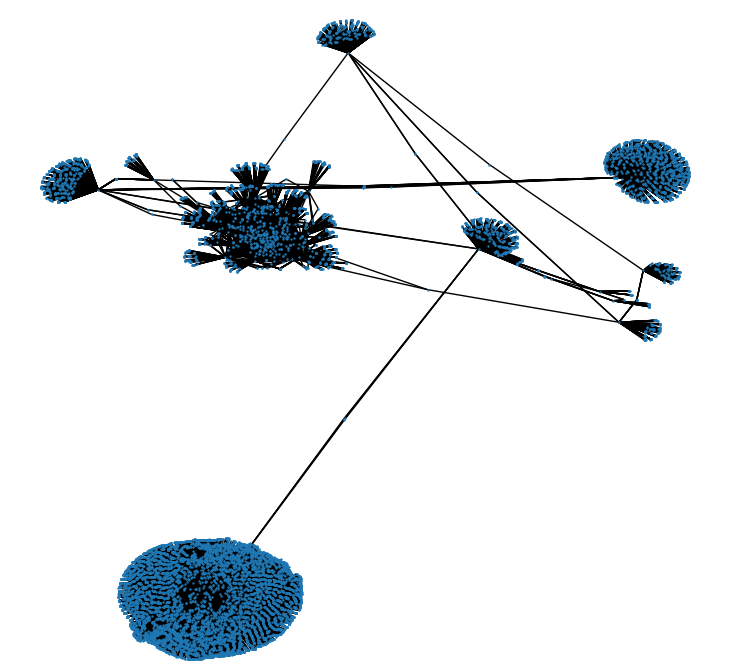
\includegraphics[scale=0.75]{net25.png}
        \caption{Red a estudiar con 25\% de los enlaces}
        \label{fig:net25}
    \end{figure}

    \begin{figure}
        \centering
        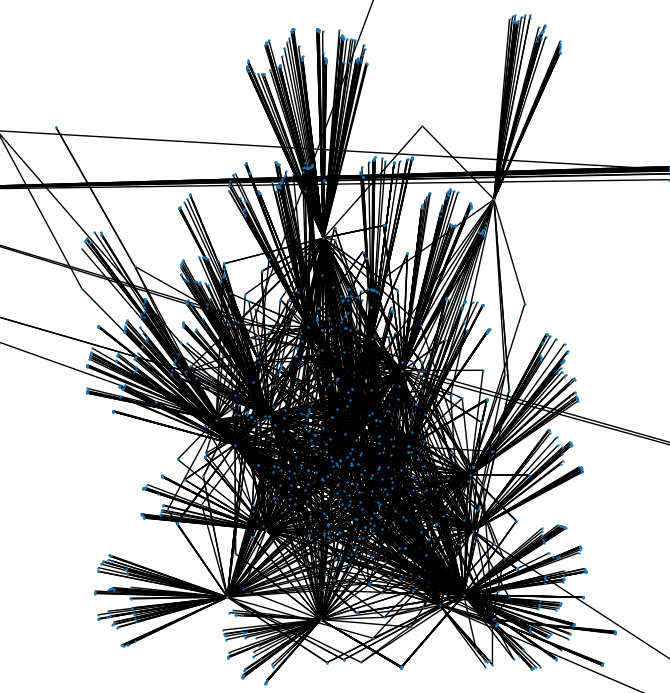
\includegraphics[width=\textwidth]{net25-detail.png}
        \caption{Detalle del componente gigante de la red a 25\%}
        \label{fig:net25detail}
    \end{figure}

    \begin{figure}
        \centering
        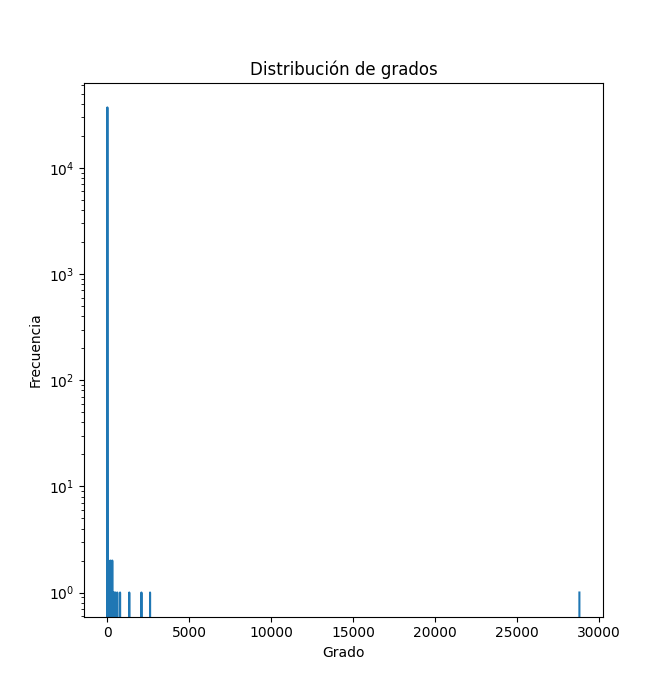
\includegraphics[scale=0.6]{degree_dist.png}
        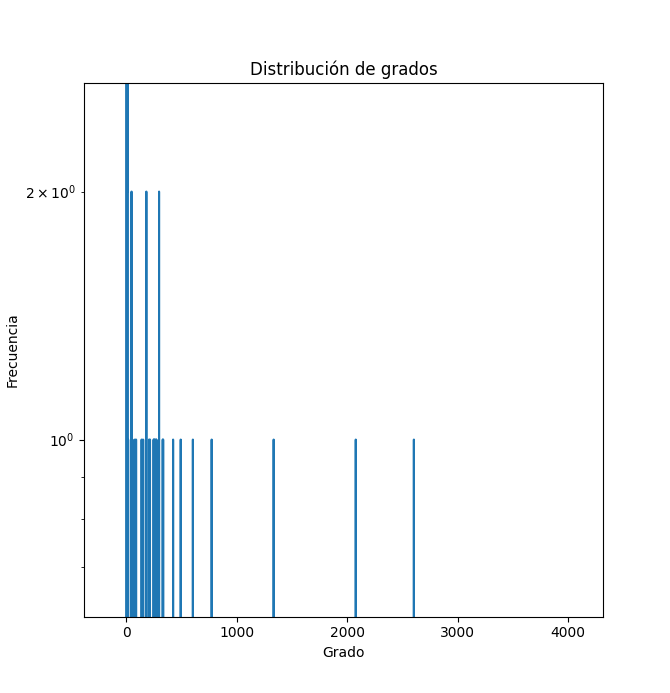
\includegraphics[scale=0.6]{degree_dist_detail.png}
        \caption{Distribución de grados. Dos escalas.}
        \label{fig:avgdeg}
    \end{figure}

    \begin{figure}
        \centering
        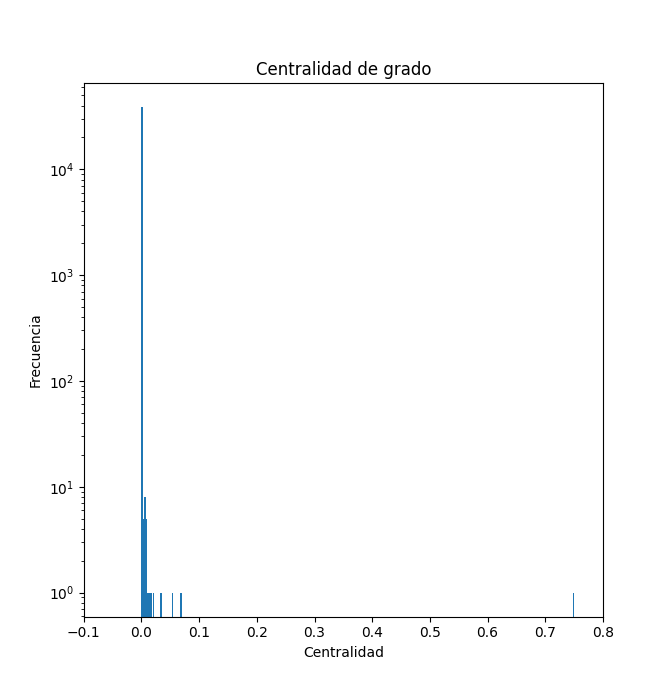
\includegraphics[scale=0.6]{degree_centrality.png}
        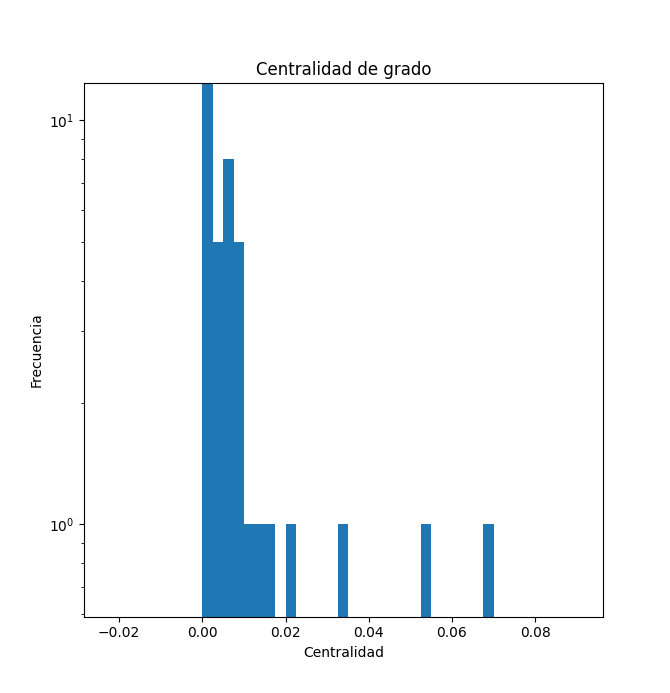
\includegraphics[scale=0.6]{degree_centrality_detail.png}
        \caption{Centralidad de grado. Dos escalas.}
        \label{fig:degcentr}
    \end{figure}

    \begin{figure}
        \centering
        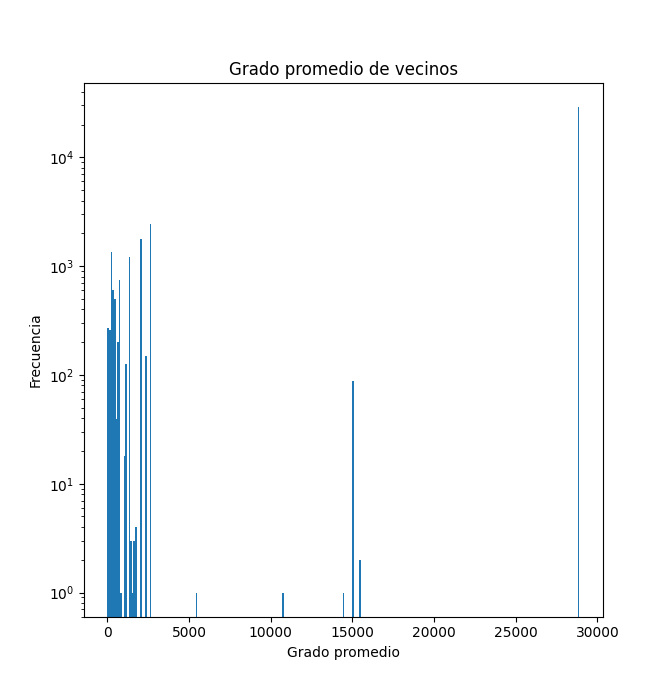
\includegraphics[scale=0.75]{avg_nei_degree.png}
        \caption{Grado promedio de vecinos}
        \label{fig:degeavgnei}
    \end{figure}

    \section*{Consideraciones}

    Varios de los datos estadísticos no sa han calculado debido a la cantidad 
    necesaria de recursos para hacerlo.Se planea usar algún tipo de servicio 
    de computación distribuida para efectuar esos cálculos en el futuro.

    Se planea estudiar la componente gigante con  la estructura menos regular.

    Falta etiquetar los nodos infectados, así como incluir en el análisis todo lo 
    relacionado a tiempo y evolución de la infección.
    
    En base a estos nuevos datos, se decidirá el modelo adecuado para modelar la red.
    
    \begin{thebibliography}{1}	
    	\bibitem{MDM} 
    	\textit{Del Rey, Á. M., Hernández, G. M., \& Queiruga-Dios, A. M. (2016). Malware Diffusion Modeling Framework. Malware Diffusion Models for Wireless Complex Networks, 1–2. doi: 10.1016/b978-0-12-802714-1.00008-6}
    	[Consultado: 9-Marzo-2020].
    	
    	\bibitem{MRB} 
    	\textit{Elisan, C. (2013). Malware, Rootkits \& Botnets: A Beginners Guide. McGraw-Hill. 55-82pp.}
    	[Consultado: 8-Marzo-2020].
    	
    	\bibitem{DES} 
    	\textit{Kotenko, I., Konovalov, A., \& Shorov, A. (2012). Discrete-Event Simulation of Botnet Protection Mechanisms. Discrete Event Simulations - Development and Applications. doi: 10.5772/50101}
    	[Consultado: 8-Marzo-2020].
    	
    	\bibitem{WMS} 
    	\textit{Liu, W., \& Zhong, S. (2017). Web malware spread modelling and optimal control strategies. Scientific Reports, 7(1). doi: 10.1038/srep42308}
    	[Consultado: 8-Marzo-2020].
    	
    	\bibitem{B} 
    	\textit{Tiirmaa-Klaar, H., Gassen, J., Gerhards-Padilla, E., \& Martini, P. (2013). Botnets. London: Springer.}
    	[Consultado: 6-Marzo-2020].
    \end{thebibliography}
\end{document}